\documentclass[10pt]{beamer}

% -------------------------------------------------------------
% Theme and Appearance
% -------------------------------------------------------------
\usetheme{CambridgeUS}
\usecolortheme{beaver}

\usepackage{booktabs}
\usepackage{graphicx}
\usepackage{xcolor}
\usepackage{caption}
\usepackage{array}
\usepackage{multirow}
\usepackage{tikz}
\usetikzlibrary{arrows.meta, positioning}

% Prevent hyperref pdfstring recursion in metadata
\pdfstringdefDisableCommands{%
  \def\\{}%
  \def\textbf#1{#1}%
  \def\small{}%
  \def\footnotesize{}%
  \def\scriptsize{}%
  \def\large{}%
  \def\Large{}%
  \def\begin#1{}%
  \def\end#1{}%
  \def\tabular#1{}%
  \def\endtabular{}%
  \def\vspace#1{}%
  \def\hspace#1{}%
}

% Remove default navigation symbols
\setbeamertemplate{navigation symbols}{}

% Color customizations matching reference style
\definecolor{svecRed}{RGB}{160, 20, 30}
\definecolor{cardBg}{RGB}{248, 249, 250}
\definecolor{cardBorder}{RGB}{200, 205, 210}

\setbeamercolor{frametitle}{fg=svecRed,bg=white}
\setbeamercolor{title}{fg=svecRed}
\setbeamercolor{item}{fg=svecRed}
\setbeamercolor{subitem}{fg=svecRed}
\setbeamercolor{structure}{fg=svecRed}

% -------------------------------------------------------------
% Custom Clean Footer (Reference Format)
% -------------------------------------------------------------
\setbeamertemplate{footline}{
  \leavevmode%
  \hbox{%
  \begin{beamercolorbox}[wd=.333333\paperwidth,ht=2.25ex,dp=1ex,center]{author in head/foot}%
    \usebeamerfont{author in head/foot}\textbf{ROADGUARD / TEAM}
  \end{beamercolorbox}%
  \begin{beamercolorbox}[wd=.333333\paperwidth,ht=2.25ex,dp=1ex,center]{title in head/foot}%
    \usebeamerfont{title in head/foot}\textbf{RoadGuard}
  \end{beamercolorbox}%
  \begin{beamercolorbox}[wd=.333333\paperwidth,ht=2.25ex,dp=1ex,right]{date in head/foot}%
    \usebeamerfont{date in head/foot}September 2026\hspace*{1.5em}
    \insertframenumber{} / \inserttotalframenumber\hspace*{2ex} 
  \end{beamercolorbox}}%
  \vskip0pt%
}

% -------------------------------------------------------------
% Presentation Title and Metadata (Protected with texorpdfstring)
% -------------------------------------------------------------
\title[RoadGuard]{\texorpdfstring{\textbf{RoadGuard: An Explainable Deep Learning-Based Road Damage Assessment and Intelligent Maintenance Prioritization System}}{RoadGuard: Road Damage Assessment and Prioritization}}
\subtitle{\texorpdfstring{Major Project Review -- I}{Major Project Review - I}}

\author[ROADGUARD / TEAM]{%
\texorpdfstring{%
\footnotesize
\begin{tabular}{cc}
Student 1: \textbf{Ch Satyanarayana} (23A81A4383) & Student 2: \textbf{G S S Priya} (23A81A4394) \\
Student 3: \textbf{A J S Prasanna} (23A81A4373) & Student 4: \textbf{G Nikhil} (23A85A4309)
\end{tabular} \\[0.4em]
{\small Project Guide: \textbf{Dr. G Venkata Lakshmi}}%
}{Ch Satyanarayana, G S S Priya, A J S Prasanna, G Nikhil}%
}

\institute[SVEC]{%
\texorpdfstring{%
\scriptsize
Department of Artificial Intelligence \& Machine Learning \\
Sri Vasavi Engineering College (Autonomous) \\
Pedatadepalli, Tadepalligudem, Andhra Pradesh, India%
}{Department of AIML, Sri Vasavi Engineering College}%
}

\date[September 2026]{September 2026}

% -------------------------------------------------------------
% Document Slides
% -------------------------------------------------------------
\begin{document}

% =============================================================
% SLIDE 1 — TITLE
% =============================================================
\begin{frame}[plain]
    \titlepage
\end{frame}

% =============================================================
% SLIDE 2 — MAJOR PROJECT REVIEW-I CONTENTS
% =============================================================
\begin{frame}{Major Project Review -- I Contents}
    \begin{columns}[t]
        \begin{column}{0.48\textwidth}
            \begin{itemize}
                \setlength{\itemsep}{0.55em}
                \item \textbf{1. Abstract}
                \item \textbf{2. Introduction}
                \item \textbf{3. Literature Survey}
                \item \textbf{4. Problem Statement in Existing System}
                \item \textbf{5. Proposed System}
                \item \textbf{6. Objectives}
            \end{itemize}
        \end{column}
        \begin{column}{0.52\textwidth}
            \begin{itemize}
                \setlength{\itemsep}{0.55em}
                \item \textbf{7. Project Domain}
                \item \textbf{8. Requirement Analysis}
                \begin{itemize}
                    \item 8.1 Functional Requirements
                    \item 8.2 Non-Functional Requirements
                    \item 8.3 Software Requirements
                    \item 8.4 Hardware Requirements
                \end{itemize}
                \item \textbf{9. System Architecture}
                \item \textbf{10. Methodology}
            \end{itemize}
        \end{column}
    \end{columns}
\end{frame}

% =============================================================
% SLIDE 3 — ABSTRACT
% =============================================================
\begin{frame}{Abstract}
    RoadGuard is an AI-based road infrastructure assessment and maintenance prioritization system designed to automate the detection, analysis, and management of road defects. The proposed system processes road images or videos captured using mobile devices or vehicle-mounted cameras and uses a deep learning-based object detection model to identify defects such as potholes, longitudinal cracks, transverse cracks, alligator cracks, and surface damage. The detected defects are analyzed to estimate their severity based on damage type, size, and defect density. GPS coordinates are associated with each detected defect to identify the corresponding road segment and determine its road type and jurisdiction using a road-authority mapping database. A maintenance-priority model then generates a priority score based on damage severity, defect concentration, road importance, location risk, and repeated reports. The results are stored in a database and visualized through an interactive map and authority dashboard, allowing responsible departments to identify critical road segments and manage maintenance activities efficiently.
\end{frame}

% =============================================================
% SLIDE 4 — INTRODUCTION
% =============================================================
\begin{frame}{Introduction}
    \begin{itemize}
        \setlength{\itemsep}{0.7em}
        \item \textbf{Road Infrastructure Deterioration:} Transportation roadway networks deteriorate continuously due to heavy vehicular traffic loading, weathering, temperature variations, and material fatigue.
        \item \textbf{Pavement Distress Categories:} Common surface defects include potholes, longitudinal cracks, transverse cracks, complex alligator cracking, and progressive surface ravelling.
        \item \textbf{Need for Automated Inspection:} Traditional manual road inspections rely on human visual surveys, which are inherently labor-intensive, slow, hazardous, and subject to observer subjectivity.
        \item \textbf{Role of AI \& Computer Vision:} Deep convolutional neural networks offer powerful opportunities to automate high-resolution pavement distress detection from optical camera imagery.
        \item \textbf{Motivation for RoadGuard:} RoadGuard advances beyond isolated visual distress detection by establishing an integrated framework for severity estimation, geospatial mapping, and automated maintenance prioritization.
    \end{itemize}
\end{frame}

% =============================================================
% SLIDE 5 — LITERATURE SURVEY
% =============================================================
\begin{frame}[shrink=4]{Literature Survey}
    \begin{table}
        \centering
        \footnotesize
        \caption{Summary of representative pavement distress detection methods}
        \begin{tabular}{@{}p{0.9cm}p{2.3cm}p{2.5cm}p{2.4cm}p{2.3cm}@{}}
            \toprule
            \textbf{Year} & \textbf{Author / Work} & \textbf{Approach} & \textbf{Contribution} & \textbf{Key Limitation} \\
            \midrule
            2018 & Traditional Vision & Canny edge detection, Otsu thresholding & Handcrafted morphological crack extraction & Highly sensitive to shadows, lighting, and textures \\
            \addlinespace[0.3em]
            2019 & Zou et al. \newline (DeepCrack) & Hierarchical deep CNN multi-scale fusion & Multi-scale feature integration for crack segmentation & High false positives on dark shadows and stains \\
            \addlinespace[0.3em]
            2021 & Chen et al. \newline (DeepLabv3+) & Atrous Spatial Pyramid Pooling (ASPP) & Captures multi-scale contextual semantic cues & Discontinuous boundaries on thin, low-contrast cracks \\
            \addlinespace[0.3em]
            2021 & Arya et al. \newline (GRDDC) & Multi-country deep object detection & Large multi-national road damage benchmark & Bounding boxes only; lacks severity \& GIS mapping \\
            \addlinespace[0.3em]
            2024 & Zhang et al. \newline (\textbf{Base Paper}) & DARNet: Xception + CFASPP + DAAM + REM & Distress-aware attention with boundary refinement & Standalone detection; lacks severity, GPS, \& priority \\
            \bottomrule
        \end{tabular}
    \end{table}
\end{frame}

% =============================================================
% SLIDE 6 — LITERATURE SURVEY: BASE PAPER
% =============================================================
\begin{frame}{Literature Survey: Base Paper}
    \textbf{Base Paper:} \textit{Automated Pavement Distress Detection Based on Convolutional Neural Network} \\
    \textbf{Authors:} Jinhe Zhang, Shangyu Sun, Weidong Song, Yuxuan Li, Qiaoshuang Teng (\textit{IEEE Access}, 2024)
    \vspace{0.4em}
    \begin{itemize}
        \setlength{\itemsep}{0.45em}
        \item \textbf{Objective:} Develop an end-to-end convolutional neural network (DARNet) to accurately detect and segment pavement distress from road imagery.
        \item \textbf{Approach:} Encoder-decoder semantic segmentation architecture utilizing an Xception backbone with multi-scale contextual feature fusion.
        \item \textbf{Main Contribution:} Mitigates crack fragmentation and blurred boundaries in complex asphalt textures through dynamic attention and edge refinement.
        \item \textbf{Important Techniques:}
        \begin{itemize}
            \item \textit{CFASPP Module:} Cross-Feature ASPP capturing multi-scale receptive fields.
            \item \textit{DAAM Module:} Distress-Aware Attention dynamically weighting defect morphology.
            \item \textit{REM \& WCEL:} Refinement Extraction Module and Weighted Cross-Entropy Loss.
        \end{itemize}
        \item \textbf{Limitation:} Focuses strictly on pixel-level distress extraction without estimating physical severity, GPS localization, or maintenance priority.
        \item \textbf{Relevance to RoadGuard:} Provides the core deep-learning computer vision foundation that RoadGuard extends into a full decision-support system.
    \end{itemize}
\end{frame}

% =============================================================
% SLIDE 7 — PROBLEM STATEMENT IN EXISTING SYSTEM
% =============================================================
\begin{frame}{Problem Statement in Existing System}
    \begin{itemize}
        \setlength{\itemsep}{0.45em}
        \item \textbf{Manual Inspection Limitations:} Traditional monitoring depends on manual visual surveys and citizen complaints, which are labor-intensive, hazardous, and slow to mobilize.
        \item \textbf{Scalability Bottlenecks:} Municipal and highway networks expand rapidly, making periodic human visual inspection impractical across vast road corridors.
        \item \textbf{Subjectivity \& Inconsistency:} Visual condition rating by human inspectors is subjective, resulting in inconsistent distress severity grading and repair delays.
        \item \textbf{Isolated Image-Based Models:} Existing deep-learning systems output only raw bounding boxes or masks without quantifying physical severity or cluster density.
        \item \textbf{Lack of Integrated Maintenance Prioritization:} Detections are rarely linked to GPS coordinates, road importance, administrative jurisdictions, or repair triage.
    \end{itemize}
    \vspace{0.3em}
    \begin{block}{\textbf{Problem Statement}}
        \footnotesize
        Existing road inspection lacks an integrated, objective, and scalable system that can automatically detect multi-class pavement distress, assess damage severity, map geographic locations and jurisdictions, and intelligently prioritize maintenance interventions.
    \end{block}
\end{frame}

% =============================================================
% SLIDE 8 — PROPOSED SYSTEM
% =============================================================
\begin{frame}{Proposed System: RoadGuard}
    \begin{center}
    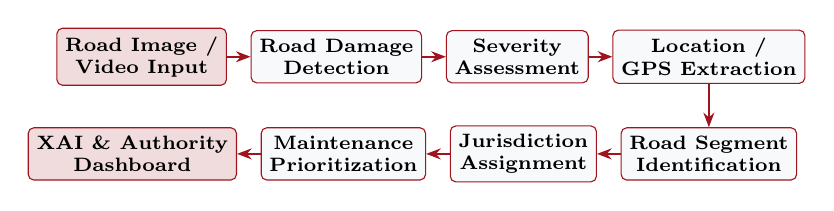
\begin{tikzpicture}[
        node distance=0.4cm and 0.3cm,
        box/.style={draw=svecRed, fill=cardBg, rounded corners=2pt, font=\scriptsize\bfseries, align=center, inner sep=3pt, minimum height=0.6cm},
        arr/.style={-{Stealth[scale=0.8]}, thick, color=svecRed}
    ]
        % Row 1
        \node[box, fill=svecRed!15] (b1) {Road Image / \\ Video Input};
        \node[box, right=of b1] (b2) {Road Damage \\ Detection};
        \node[box, right=of b2] (b3) {Severity \\ Assessment};
        \node[box, right=of b3] (b4) {Location / \\ GPS Extraction};
        
        % Row 2
        \node[box, below=0.55cm of b4] (b5) {Road Segment \\ Identification};
        \node[box, left=of b5] (b6) {Jurisdiction \\ Assignment};
        \node[box, left=of b6] (b7) {Maintenance \\ Prioritization};
        \node[box, left=of b7, fill=svecRed!15] (b8) {XAI \& Authority \\ Dashboard};
        
        % Connectors
        \draw[arr] (b1) -- (b2);
        \draw[arr] (b2) -- (b3);
        \draw[arr] (b3) -- (b4);
        \draw[arr] (b4) -- (b5);
        \draw[arr] (b5) -- (b6);
        \draw[arr] (b6) -- (b7);
        \draw[arr] (b7) -- (b8);
    \end{tikzpicture}
    \end{center}
    \vspace{0.2em}
    \begin{itemize}
        \setlength{\itemsep}{0.35em}
        \item \textbf{End-to-End Automation:} Seamless pipeline connecting optical road imagery directly to municipal maintenance work orders.
        \item \textbf{Multi-Class Defect Detection:} Accurately localizes potholes, longitudinal cracks, transverse cracks, and alligator cracks.
        \item \textbf{Objective Severity Scoring:} Evaluates damage dimensions, surface coverage, and localized defect density.
        \item \textbf{Geospatial Asset Linking:} Maps GPS coordinates to road segments, functional road categories, and responsible departments.
        \item \textbf{Explainable Prioritization:} Delivers transparent visual heatmaps and ranked maintenance schedules on an interactive dashboard.
    \end{itemize}
\end{frame}

% =============================================================
% SLIDE 9 — OBJECTIVES
% =============================================================
\begin{frame}{Objectives}
    \begin{itemize}
        \setlength{\itemsep}{0.65em}
        \item \textbf{O1:} Develop a deep learning-based model to automatically detect and classify pavement distress from road imagery.
        \item \textbf{O2:} Identify multiple defect categories including potholes, longitudinal cracks, transverse cracks, and alligator cracks.
        \item \textbf{O3:} Formulate an objective damage severity assessment model based on defect type, physical size, and local density.
        \item \textbf{O4:} Integrate GPS coordinate extraction to localize detected damage instances accurately along surveyed road corridors.
        \item \textbf{O5:} Implement an automated road-segment and jurisdiction mapping module to identify responsible maintenance departments.
        \item \textbf{O6:} Develop an intelligent maintenance priority model balancing damage severity, defect concentration, road type, and risk.
        \item \textbf{O7:} Provide explainable AI visualizations and an interactive GIS dashboard for transparent maintenance decision-making.
    \end{itemize}
\end{frame}

% =============================================================
% SLIDE 10 — PROJECT DOMAIN
% =============================================================
\begin{frame}{Project Domain}
    \textbf{\large Primary Domain:}
    \vspace{0.2em}
    \begin{itemize}
        \item \textbf{Artificial Intelligence \& Machine Learning}
    \end{itemize}
    \vspace{0.4em}
    \textbf{\large Sub-Domains \& Technical Focus Areas:}
    \vspace{0.2em}
    \begin{itemize}
        \setlength{\itemsep}{0.45em}
        \item \textbf{Deep Learning:} Convolutional neural networks and attention architectures for robust spatial feature representation.
        \item \textbf{Computer Vision:} Automated object detection, distress localization, and defect boundary segmentation.
        \item \textbf{Digital Image Processing:} Illumination correction, adaptive histogram equalization, and morphological edge analysis.
        \item \textbf{Geospatial Analysis \& GIS:} GPS telemetry extraction, spatial indexing, road-segment matching, and boundary attribution.
        \item \textbf{Explainable AI (XAI):} Visual attention heatmaps and transparent feature attribution for verifiable engineering decisions.
        \item \textbf{Intelligent Infrastructure Monitoring:} Data-driven road condition assessment, risk modeling, and predictive repair triage.
    \end{itemize}
\end{frame}

% =============================================================
% SLIDE 11 — REQUIREMENT ANALYSIS: FUNCTIONAL REQUIREMENTS
% =============================================================
\begin{frame}{Requirement Analysis: Functional Requirements}
    \begin{itemize}
        \setlength{\itemsep}{0.4em}
        \item \textbf{FR1 -- Image \& Video Input:} Ingest optical road imagery and video streams from vehicle cameras and mobile survey units.
        \item \textbf{FR2 -- Image Preprocessing:} Perform automated noise suppression, illumination normalization, and image enhancement.
        \item \textbf{FR3 -- Damage Detection:} Detect and classify potholes, longitudinal cracks, transverse cracks, and alligator cracks.
        \item \textbf{FR4 -- Severity Assessment:} Quantify defect severity levels based on bounding dimensions, surface area, and cluster density.
        \item \textbf{FR5 -- Location Association:} Extract and associate spatial latitude and longitude coordinates with detected defects.
        \item \textbf{FR6 -- Road Segment Identification:} Match GPS coordinates to specific road corridors and functional road hierarchies.
        \item \textbf{FR7 -- Jurisdiction Mapping:} Route identified distress points to the responsible administrative authority (e.g., Municipality, PWD, NHAI).
        \item \textbf{FR8 -- Maintenance Prioritization:} Compute multi-factor maintenance priority scores based on damage, road type, and risk.
        \item \textbf{FR9 -- XAI Visualization \& Dashboard:} Generate visual explanation heatmaps and display interactive map analytics for authorities.
    \end{itemize}
\end{frame}

% =============================================================
% SLIDE 12 — REQUIREMENT ANALYSIS: NON-FUNCTIONAL REQUIREMENTS
% =============================================================
\begin{frame}{Requirement Analysis: Non-Functional Requirements}
    \begin{itemize}
        \setlength{\itemsep}{0.48em}
        \item \textbf{NFR1 -- Accuracy:} Achieve high precision, recall, and mAP in identifying diverse distress types across varied road surfaces.
        \item \textbf{NFR2 -- Reliability:} Ensure consistent defect detection under challenging lighting, heavy shadows, and weathered textures.
        \item \textbf{NFR3 -- Performance:} Deliver low-latency image inference suitable for rapid batch processing and mobile survey units.
        \item \textbf{NFR4 -- Scalability:} Support expanding road networks, high volumes of survey frames, and multi-agency user access.
        \item \textbf{NFR5 -- Usability:} Provide an intuitive, interactive dashboard interface for municipal engineers with minimal technical overhead.
        \item \textbf{NFR6 -- Explainability:} Offer transparent visual evidence to ensure domain engineers can understand and verify automated outputs.
        \item \textbf{NFR7 -- Security:} Ensure secure storage, integrity of geotagged survey reports, and role-based access for authorities.
        \item \textbf{NFR8 -- Maintainability:} Maintain a loosely coupled modular architecture allowing independent model updates and dataset retraining.
    \end{itemize}
\end{frame}

% =============================================================
% SLIDE 13 — REQUIREMENT ANALYSIS: SOFTWARE & HARDWARE REQUIREMENTS
% =============================================================
\begin{frame}{Requirement Analysis: Software \& Hardware Requirements}
    \begin{columns}[t]
        \begin{column}{0.48\textwidth}
            \textbf{\large Software Requirements}
            \vspace{0.4em}
            \begin{itemize}
                \setlength{\itemsep}{0.45em}
                \item \textbf{Operating System:} \\ Windows 10 / 11, Linux (Ubuntu)
                \item \textbf{Programming Language:} \\ Python 3.10+
                \item \textbf{Deep Learning Frameworks:} \\ PyTorch, Torchvision, Ultralytics YOLO
                \item \textbf{Computer Vision:} \\ OpenCV, Pillow, NumPy
                \item \textbf{Geospatial \& GIS Tools:} \\ GeoPandas, Shapely, Folium / Leaflet
                \item \textbf{Database Management:} \\ PostgreSQL with PostGIS / SQLite
                \item \textbf{Web Framework \& UI:} \\ FastAPI / Flask, React / Streamlit
            \end{itemize}
        \end{column}
        \begin{column}{0.48\textwidth}
            \textbf{\large Hardware Requirements}
            \vspace{0.4em}
            \begin{itemize}
                \setlength{\itemsep}{0.45em}
                \item \textbf{Processor (CPU):} \\ Intel Core i5 / i7 (8th Gen+) or AMD Ryzen 5 / 7
                \item \textbf{Graphics Card (GPU):} \\ NVIDIA GeForce GTX 1650 / RTX 3060 (4GB+ VRAM) with CUDA support
                \item \textbf{System Memory (RAM):} \\ 16 GB DDR4 RAM
                \item \textbf{Storage:} \\ 512 GB NVMe SSD (fast dataset and model weight I/O)
                \item \textbf{Capture Devices:} \\ High-resolution mobile camera (12MP+) / Vehicle-mounted dashcam
                \item \textbf{GPS Module:} \\ Built-in smartphone GPS / GNSS receiver
            \end{itemize}
        \end{column}
    \end{columns}
\end{frame}

% =============================================================
% SLIDE 14 — SYSTEM ARCHITECTURE
% =============================================================
\begin{frame}{System Architecture}
    \begin{center}
    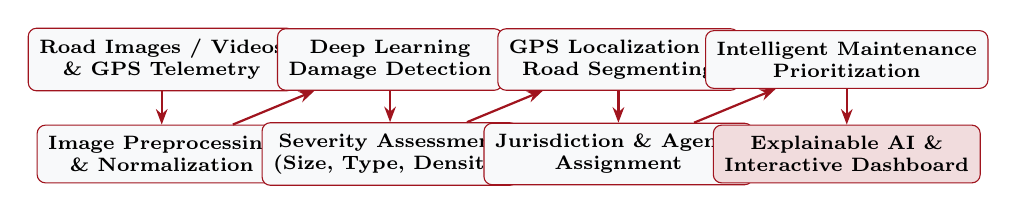
\begin{tikzpicture}[
        box/.style={draw=svecRed, fill=cardBg, rounded corners=3pt, font=\scriptsize\bfseries, align=center, inner sep=4pt, minimum width=2.4cm, minimum height=0.55cm},
        arr/.style={-{Stealth[scale=0.85]}, thick, color=svecRed}
    ]
        % Column 1: Input & Preprocessing
        \node[box] (inp) at (0, 1.2) {Road Images / Videos \\ \& GPS Telemetry};
        \node[box] (prep) at (0, 0) {Image Preprocessing \\ \& Normalization};
        
        % Column 2: Detection & Severity
        \node[box] (det) at (2.9, 1.2) {Deep Learning \\ Damage Detection};
        \node[box] (sev) at (2.9, 0) {Severity Assessment \\ (Size, Type, Density)};
        
        % Column 3: Geospatial & Jurisdiction
        \node[box] (geo) at (5.8, 1.2) {GPS Localization \& \\ Road Segmenting};
        \node[box] (jur) at (5.8, 0) {Jurisdiction \& Agency \\ Assignment};
        
        % Column 4: Decision & Presentation
        \node[box] (pri) at (8.7, 1.2) {Intelligent Maintenance \\ Prioritization};
        \node[box, fill=svecRed!15] (dash) at (8.7, 0) {Explainable AI \& \\ Interactive Dashboard};
        
        % Sequential pipeline arrows
        \draw[arr] (inp) -- (prep);
        \draw[arr] (prep) -- (det);
        \draw[arr] (det) -- (sev);
        \draw[arr] (sev) -- (geo);
        \draw[arr] (geo) -- (jur);
        \draw[arr] (jur) -- (pri);
        \draw[arr] (pri) -- (dash);
    \end{tikzpicture}
    \end{center}
    \vspace{0.4em}
    \begin{itemize}
        \item \textbf{Input Tier:} Ingests optical roadway frames and GPS coordinate metadata.
        \item \textbf{Vision Tier:} Performs defect detection and quantitative physical severity scoring.
        \item \textbf{Spatial Tier:} Associates defects with road segments and responsible authorities.
        \item \textbf{Decision Tier:} Ranks maintenance urgency and visualizes data on an interactive GIS console.
    \end{itemize}
\end{frame}

% =============================================================
% SLIDE 15 — SYSTEM ARCHITECTURE: COMPONENTS
% =============================================================
\begin{frame}{System Architecture: Components}
    \begin{itemize}
        \setlength{\itemsep}{0.4em}
        \item \textbf{Data Acquisition \& Ingestion Module:} Captures and ingests road imagery and video frames from mobile survey units, vehicular dashcams, and citizen reports.
        \item \textbf{Image Preprocessing Module:} Performs noise reduction, illumination correction, and adaptive contrast enhancement to standardize raw visual inputs.
        \item \textbf{Deep Learning Detection Module:} Utilizes deep convolutional feature extractors to detect, classify, and localize diverse road distress categories.
        \item \textbf{Severity Assessment Module:} Evaluates damage dimensions, defect density, and surface coverage to assign objective severity levels.
        \item \textbf{Geospatial \& Road-Segment Module:} Extracts GPS metadata to accurately match distress instances with municipal road corridors and road classifications.
        \item \textbf{Jurisdiction Assignment Module:} Automatically routes verified defects to the responsible agency (e.g., Municipality, PWD, NHAI) based on spatial boundaries.
        \item \textbf{Maintenance Prioritization Engine:} Ranks repair urgency using a multi-factor scoring model combining severity, road hierarchy, and location risk.
        \item \textbf{Explainable AI \& Dashboard Module:} Generates visual explanation heatmaps and provides an interactive GIS portal for engineering staff.
    \end{itemize}
\end{frame}

% =============================================================
% SLIDE 16 — METHODOLOGY
% =============================================================
\begin{frame}{Methodology}
    \begin{itemize}
        \setlength{\itemsep}{0.32em}
        \item \textbf{Stage 1 -- Data Collection:} Gather diverse pavement imagery from public benchmarks (RDD2022, Crack500) and localized mobile survey captures.
        \item \textbf{Stage 2 -- Data Preprocessing:} Normalize contrast, resize frames, apply illumination equalization, and generate data augmentations.
        \item \textbf{Stage 3 -- Road Damage Detection:} Extract multiscale visual features using deep convolutional layers to locate pavement distress areas.
        \item \textbf{Stage 4 -- Damage Classification:} Categorize detected distress into potholes, longitudinal cracks, transverse cracks, and alligator cracks.
        \item \textbf{Stage 5 -- Severity Assessment:} Quantify physical distress severity levels using bounding dimensions, segmented area, and defect concentration.
        \item \textbf{Stage 6 -- Location Association:} Extract GNSS/GPS coordinate metadata to determine exact spatial locations of defects.
        \item \textbf{Stage 7 -- Road Segment Mapping:} Align defect coordinates with municipal GIS road layers to identify road types and responsible authorities.
        \item \textbf{Stage 8 -- Maintenance Prioritization:} Calculate an objective repair priority score combining severity, traffic importance, and structural risk.
        \item \textbf{Stage 9 -- Explainable AI:} Produce saliency/attention maps to provide interpretable visual justification for model predictions.
        \item \textbf{Stage 10 -- Dashboard Telemetry:} Publish processed distress data, spatial clusters, and ranked maintenance lists to an interactive authority dashboard.
    \end{itemize}
\end{frame}

% =============================================================
% SLIDE 17 — METHODOLOGY: DETAILED WORKFLOW
% =============================================================
\begin{frame}{Methodology: Detailed Workflow}
    \begin{center}
    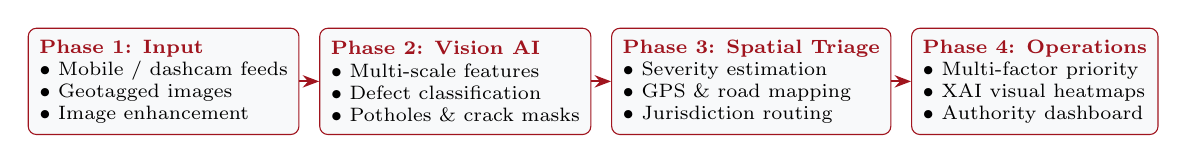
\begin{tikzpicture}[
        node distance=0.45cm and 0.25cm,
        card/.style={draw=svecRed, fill=cardBg, rounded corners=3pt, font=\scriptsize, align=left, inner sep=4pt, minimum width=2.45cm, minimum height=1.35cm},
        arr/.style={-{Stealth[scale=0.9]}, thick, color=svecRed}
    ]
        % Phase 1
        \node[card] (p1) {
            \textbf{\color{svecRed}Phase 1: Input} \\
            $\bullet$ Mobile / dashcam feeds \\
            $\bullet$ Geotagged images \\
            $\bullet$ Image enhancement
        };
        
        % Phase 2
        \node[card, right=of p1] (p2) {
            \textbf{\color{svecRed}Phase 2: Vision AI} \\
            $\bullet$ Multi-scale features \\
            $\bullet$ Defect classification \\
            $\bullet$ Potholes \& crack masks
        };
        
        % Phase 3
        \node[card, right=of p2] (p3) {
            \textbf{\color{svecRed}Phase 3: Spatial Triage} \\
            $\bullet$ Severity estimation \\
            $\bullet$ GPS \& road mapping \\
            $\bullet$ Jurisdiction routing
        };
        
        % Phase 4
        \node[card, right=of p3] (p4) {
            \textbf{\color{svecRed}Phase 4: Operations} \\
            $\bullet$ Multi-factor priority \\
            $\bullet$ XAI visual heatmaps \\
            $\bullet$ Authority dashboard
        };
        
        % Arrows
        \draw[arr] (p1) -- (p2);
        \draw[arr] (p2) -- (p3);
        \draw[arr] (p3) -- (p4);
    \end{tikzpicture}
    \end{center}
    \vspace{0.4em}
    \begin{itemize}
        \setlength{\itemsep}{0.4em}
        \item \textbf{Step 1 (Sensing \& Ingestion):} Captures continuous video or citizen photos and extracts synchronized geospatial coordinates.
        \item \textbf{Step 2 (Visual Feature Analysis):} Applies deep convolutional backbones to detect distress boundaries and classify morphological types.
        \item \textbf{Step 3 (Geospatial \& Risk Attribution):} Quantifies physical defect severity and matches damage instances to administrative road assets.
        \item \textbf{Step 4 (Actionable Maintenance Triage):} Computes repair priority rankings and publishes explainable evidence for engineering action.
    \end{itemize}
\end{frame}

% =============================================================
% SLIDE 18 — THANK YOU
% =============================================================
\begin{frame}{Thank You}
    \centering
    \vspace{0.3cm}
    {\Large \textbf{\color{svecRed}Questions \& Discussion}}
    \vspace{0.6cm}
    
    \textbf{\large Student Team:} \\
    \vspace{0.3em}
    Ch Satyanarayana \quad G S S Priya \quad A J S Prasanna \quad G Nikhil \\
    \vspace{0.6cm}
    
    \textbf{Project Guide:} \\
    \vspace{0.2em}
    Dr. G Venkata Lakshmi \\
    \vspace{0.4em}
    {\small Department of Artificial Intelligence \& Machine Learning} \\
    {\footnotesize Sri Vasavi Engineering College (Autonomous)} \\
    {\scriptsize Pedatadepalli, Tadepalligudem, Andhra Pradesh, India}
\end{frame}

\end{document}
